\section{Relay module}
\begin{figure}[H]
    \centering
    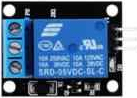
\includegraphics[angle=0, keepaspectratio=true, scale=1, width=200px, height=200px]{images/relay.jpg}
    %\caption{Caption}
\end{figure}
\subsection*{Description}
A DC relay is an electromagnetic switch. Applying a voltage across the relay terminals will close the switch which allows us to control a separate circuit.

\subsection*{Pin mapping}
This pin mapping corresponds to the pins from left to right with the module pins facing towards you.
\begin{table}[H]
    \centering
    \begin{tabular}{|c|c|c|c|c|}
    \hline
    Index &Label &Type &Name &Description\\ \hline
    0 &S &Digital input &D0 &Signal to activate relay \\ \hline
    1 &+ &Source voltage &$V+$ &Module source voltage ($5V$)\\ \hline
    2 &- &Ground &GND &\\ \hline
    \end{tabular}
    %\caption{Caption}
    %\label{tab:my_label}
\end{table}
\subsection*{Operation}
The relay is activated by setting the digital input pin D0 of the module to high. When the relay is activated there will be a short circuit between the NO (Normally open) and COM (Common) terminals. Alternatively, when the relay is not activated there is a short circuit between the NC (Normally closed) and COM (Common) terminals.
%\subsection*{Code}
%\lstinputlisting[caption=test]{laser.py}